The chosen model for the discriminative analysis is the \textit{Support Vector Machine} classifier,
an approach for classification that was developed in the computer science community in the 1990s
and that has grown in popularity since then. The SVM is a member of the family of
\textit{maximal margin classifiers}, which base its strategy in finding the hyperplane that
best separate the positive and negative instances \cite{svm_jwht}.

\subsection{Maximal Margin Classifiers}
In a \textit{p-dimensional} space, a hyperplane is a flat affine subspace of
dimension $p-1$ defined by the equation:

\begin{equation}
  \label{eq:hyperplane}
  \beta_{0} + \beta_{1}X_{1} + \beta_{2}X_{2} + \dotsc + \beta_{p}X_{p} = 0
\end{equation}

The equation defines a \textit{p-dimensional} hyperplane in the sense that if a point
$X=(X_{1}, X_{2}, \dotsc, X_{p})^{T}$ in \textit{p-dimensional} space
satisfies \ref{eq:hyperplane} then $X$ lies on the hyperplane.

If $X$ doesn't lie in the hyperplane then either:

\begin{equation}
  \label{eq:hyperplaneGreater}
  \beta_{0} + \beta_{1}X_{1} + \beta_{2}X_{2} + \dotsc + \beta_{p}X_{p} > 0
\end{equation}

\begin{center}or\end{center}

\begin{equation}
  \label{eq:hyperplaneLesser}
  \beta_{0} + \beta_{1}X_{1} + \beta_{2}X_{2} + \dotsc + \beta_{p}X_{p} < 0
\end{equation}

So the hyperplane somehow divides the \textit{p-dimensional} space into two halves. One can
easily determine on which side of the hyperplane a point lies by simply calculating the sign
of the left hand side of \ref{eq:hyperplane}.

Having a set of $n$ instances of dimension $p$, with labels
$y_{1}, y_{2}, \dotsc y_{n} \in \{-1,1\}$ and $x^{i} = (x^{i}_{1}, x^{i}_{2}, \dotsc x^{i}_{p}) \ \forall \ 1 \leq i \leq {n}$ and supposing that it is possible to construct a hyperplane that
separates the training observations perfectly according to their class labels, then a
separating hyperplane has the property that:

\begin{equation}
\beta_{0} + \beta_{1}X_{1} + \beta_{2}X_{2} + \dotsc + \beta_{p}X_{p} > 0 \ if \ y_{i} = 1
\end{equation}

\begin{center}and\end{center}

\begin{equation}
\beta_{0} + \beta_{1}X_{1} + \beta_{2}X_{2} + \dotsc + \beta_{p}X_{p} < 0 \ if \ y_{i} = -1
\end{equation}

A test observation $x^{*}$ is classified based on the sign of
$f(x^{*})=\beta_{0}+\beta_{1}x^{*}_{1} + \beta_{2}x^{*}_{2} + \dotsc + \beta_{p}x^{*}_{p}$.
If $f(x^{*})$ is positive, then it is assigned to class 1 whereas if $f(x^{*})$ is negative
then it is assigned to class -1. In addition, the magnitude of $f(x^{*})$ also contains valuable
information.
If $f(x^{*})$ is far from zero then it means that $x^{*}$ lies far from the hyperplane
whereas if $f(x^{*})$ is close to zero then $x^{*}$ is located near the hyperplane and
there is less certainty about the class of $x^{*}$.

In general, if the data can be perfectly separated using a hyperplane, then there will be an
infinite number of such hyperplanes. This is because a given separating hyperplane can usually
be shift a tiny bit up or down, or rotating without coming into contact with any of the
observations.

\begin{figure}[H]
  \centering
  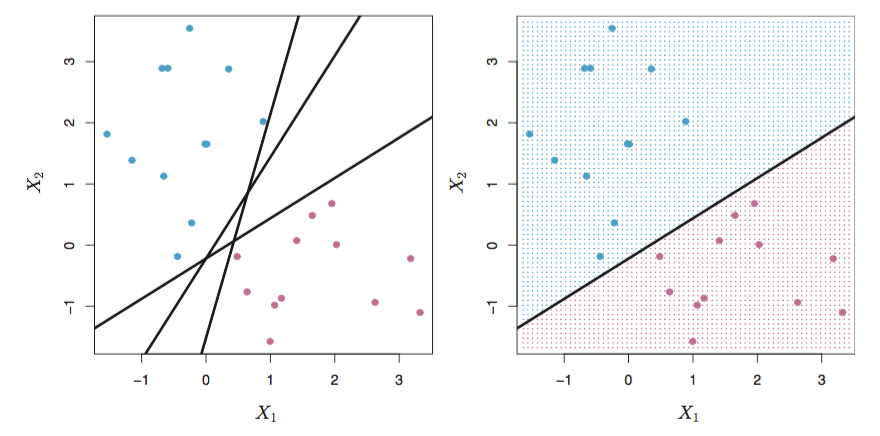
\includegraphics[width=0.8\textwidth]{files/figures/method/max-margin}
  \caption{Taken from \textit{JWHT} \cite{svm_jwht} book.
  Left: Three separating hyperplanes out of many
  possibilities. Right: Optimal Separating Hyperplane for the same dataset. A test observation
  that falls in the blue portion of the grid will be assigned to the blue class, and a test
  observation that falls in the purple portion of the grid will be assigned
  to the purple class.}
  \label{fig:maxMargin}
\end{figure}

A natural choice is the \textit{Maximal Margin Classifiers} (also known as the
\textit{Optimal Separating Hyerplane}), which is the separating hyperplane that is farthest
from the training observations. The \textit{margin} of the hyperplane is computed as the
minimal perpendicular distance to the hyperplane among all the training observations.
The maximal margin hyperplane is the separating hyperplane for which the margin is the largest.
The core idea is that a classifier that has a large margin on the training data will also
have a large margin on the test data.

\subsection{Support Vectors}

The separating hyperplane is determined by the instances of both classes that lies on the margin
of the hyperplane. These observations are known as \textit{Support Vectors}.
Observations can be interpreted as vectors in a \textit{p-dimensional} space and they
"support" the maximal
margin hyperplane in the sense that if these points were moved slightly then the maximal
margin hyperplane would move as well. The maximal margin hyperplane depends directly on the
support vectors, but not on the other observations: a movement to any of the other observations
would not affect the separating hyperplane, provided that the observation's movement does not cause
it to cross the boundary set by the margin.

\begin{figure}[H]
  \centering
  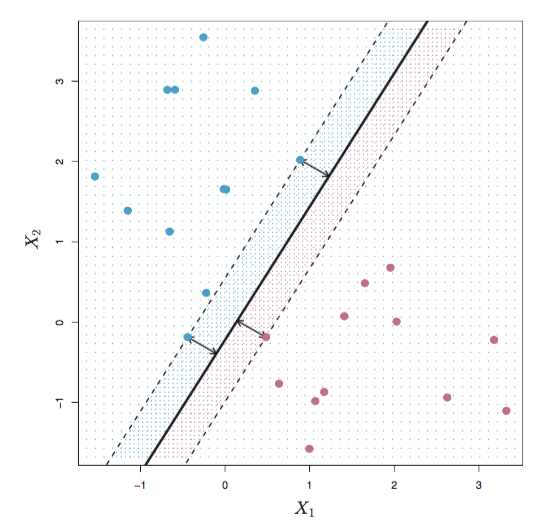
\includegraphics[width=0.4\textwidth]{files/figures/method/support-vectors}
  \caption{Taken from \textit{JWHT} \cite{svm_jwht} book. The maximal margin hyperplane
  is shown as a solid line. The margin is the distance between the solid line to either
  of the dashed lines. The two blue points and the purple point that line on the
  dashed lines are the support vectors.}
  \label{fig:maxMargin}
\end{figure}

\subsection{Problem Formulation}

It can be proven that given a set of $n$ observations of dimension $p$, the problem of
finding the \textit{Maximal Margin Hyperplane} can be posed as an optimization problem:
minimize $\| w \| = (\beta_{1}, \dotsc, \beta_{p})$.

\begin{equation}
\label{eq:svmOptimization}
w^{T}x^{*} = p\| w \|
\end{equation}

where $x^{*}$ is an observation and $p$ is the length of the projection of the observation
onto the normal vector of the hyperplane, i.e, the distance to the hyperplane.
Equation \ref{eq:svmOptimization} states that in order to maximize $p$ the norm of $w$
has to be minimized. On the other hand, the minimization problem is subject to the constraint:

\begin{equation}
  \label{eq:svmConstraint}
  y_{i} * (\beta_{0} + \beta_{1}x_{1} + \beta_{2}x_{2} + \dotsc + \beta_{p}x_{p}) > 0 \ \forall \ 1 \leq i \leq {n}
\end{equation}

Equation \ref{eq:svmConstraint} can be easily derived from \ref{eq:hyperplaneGreater} and
\ref{eq:hyperplaneLesser}.  This context matches the necessary conditions to apply
the \textit{Lagrange Multipliers} technique, to get this problem into a form
that can be solved analytically.

In practice, real data is scarcely ever completely linearly separable
and there is a trade off between
minimizing $\| w \|$ (i.e separating the instances by the largest possible margin)
and satisfying the constraint imposed over every
observation to lie on the right side of the hyperplane.
The desired hyperplane is one which separates correctly the vast majority of the observations and
at the same time it separates them by the largest margin. For this reason, when training an
\textit{SVM} classifier an additional parameter $C$ is passed as argument to the training
method in order to prioritize one problem over the other. A bigger $C$ favors the correctly
classification of the instances, while a smaller one favors the minimization of $\| w \|$
and thus finding the hyperplane with the largest margin for most of the instances.

(Agregar foto del efecto del parámetro C)

(Agregar la aclaración de que no vamos a comentar acerca de los kernels no lineales porque
no se usan)
